% Nityanand Misra: LaTeX code to typeset a book in Sanskrit
% Copyright (C) 2016 Nityanand Misra
%
% This program is free software: you can redistribute it and/or modify it under
% the terms of the GNU General Public License as published by the Free Software
% Foundation, either version 3 of the License, or (at your option) any later
% version.
%
% This program is distributed in the hope that it will be useful, but WITHOUT
% ANY WARRANTY; without even the implied warranty of  MERCHANTABILITY or FITNESS
% FOR A PARTICULAR PURPOSE. See the GNU General Public License for more details.
%
% You should have received a copy of the GNU General Public License along with
% this program.  If not, see <http://www.gnu.org/licenses/>.

\documentclass[12pt]{article}
\usepackage[paperheight=270mm,paperwidth=384mm,margin=0in]{geometry}
\usepackage[dvipsnames,prologue,table]{pstricks}
\usepackage{pst-all}
\usepackage{graphicx}
\usepackage{rotating}
\usepackage{color}
\usepackage[ISBN=978-81-92385-64-8]{ean13isbn}
\usepackage{polyglossia}
\setmainlanguage{hindi}
\setotherlanguage{english}
\setmainfont[Script=Devanagari]{Sanskrit 2003 NM}
\newfontfamily\devanagarifont[Script=Devanagari]{Sanskrit 2003 NM}
\newfontfamily{\engtextfont}{Charis SIL}
\usepackage{hyperref}
\hypersetup{
	pdfstartview={XYZ null null 1},
	bookmarks=false
}
\setlength{\parindent}{0pt}
\begin{document}
\pagecolor{Maroon}
\pagestyle{empty}
\psset{unit=1in}
\begin{pspicture}(384mm,270mm)
\DeclareFixedFont{\PT}{T1}{ppl}{b}{it}{0.5in}
\DeclareFixedFont{\PTsmall}{T1}{ppl}{b}{it}{0.4in}
\DeclareFixedFont{\PTsmallest}{T1}{ppl}{b}{it}{0.3in}
\DeclareFixedFont{\PTtext}{T1}{ppl}{b}{it}{11pt}
\DeclareFixedFont{\Logo}{T1}{pbk}{m}{n}{0.3in}
\newsavebox\IBox
\sbox\IBox{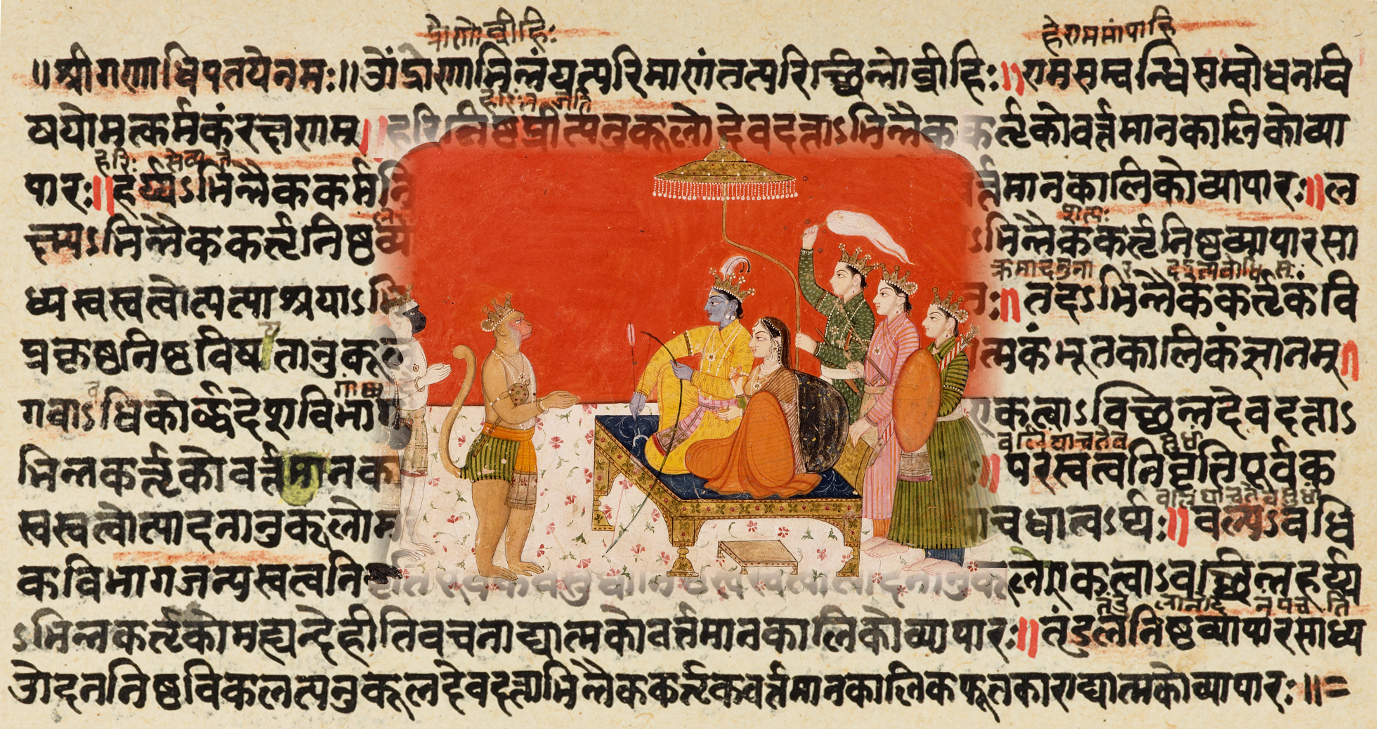
\includegraphics[width=160mm]{folio2.jpg}}
\rput[lb](213mm,53mm){\usebox\IBox}

\rput[lb](204mm,209mm){\parbox{18cm}{\centering\fontsize{28}{42}\selectfont\color{white}{\engtextfont \textbf{Adhyātmarāmāyaṇe’pāṇinīya–}}}}
\rput[lb](204mm,195mm){\parbox{18cm}{\centering\fontsize{28}{42}\selectfont\color{white}{\engtextfont \textbf{prayogāṇāṃ Vimarśaḥ}}}}
\rput[lb](204mm,170mm){\parbox{18cm}{\centering\fontsize{20}{30}\selectfont\color{white}{\engtextfont \textbf{Ācārya Giridharalāla Miśra Prajñācakṣu}}}}
\rput[lb](204mm,163mm){\parbox{18cm}{\centering\fontsize{14}{21}\selectfont\color{white}{\engtextfont known later as}}}
\rput[lb](204mm,152mm){\parbox{18cm}{\centering\fontsize{18}{27}\selectfont\color{white}{\engtextfont Jagadguru Rāmānandācārya Svāmī Rāmabhadrācārya}}}
\rput[lb](204mm,35mm){\parbox{18cm}{\centering\fontsize{14}{21}\selectfont\color{white}{\engtextfont Edited with notes by}}}
\rput[lb](204mm,25mm){\parbox{18cm}{\centering\fontsize{18}{27}\selectfont\color{white}{\engtextfont \textbf{Nityānanda Miśra}}}}

\rput[b](192mm,2.0,0.75)
{
\begin{turn} {-90}
{
\fontsize{22}{36}\selectfont\color{white}{\engtextfont \textbf{Adhyātmarāmāyaṇe’pāṇinīyaprayogāṇāṃ Vimarśaḥ}}
}
\end{turn}
}

\newsavebox\logobox
\sbox\logobox{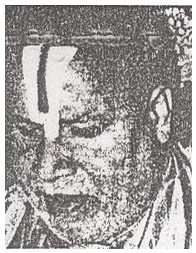
\includegraphics[width=.75in]{stpsn.jpg}}
\rput[lb](181.75mm,15mm){\usebox\logobox}

\rput[lb](20mm,155mm){\parbox{14cm}{\fontsize{13}{18}\selectfont\color{white}{\engtextfont Originally authored in 1981, this book is the PhD dissertation of the polyglot and polymath Hindū saint Jagadguru Rāmānandācārya Svāmī Rāmabhadrācārya (then known as Ācārya Giridharalāla Miśra Prajñācakṣu). Svāmī Rāmabhadrācārya is the founder of Tulsi Peeth, a social and religious organization at Chitrakoot, and the founder and lifelong chancellor of a university for the differently abled at Chitrakoot. Without eyesight since the age of two months and without formal education till the age of 17 years, Svāmī Rāmabhadrācārya speaks 22 languages and has authored more than 100 books in Sanskrit and Hindi. In this work, Svāmī Rāmabhadrācārya has examined ‘non-Pāṇinian’ usages in the \textit{Adhyātma Rāmāyaṇa} using traditional and novel methods drawing from the Pāṇinian framework. This edition of the book is edited and annotated by Nityānanda Miśra, a Sanskrit enthusiast who works in the investment banking industry at Mumbai. He is an initiated disciple of Svāmī Rāmabhadrācārya.}}}

\rput[lb](20mm,130mm){\parbox{14cm}{\fontsize{13}{21}\selectfont\color{white}{\engtextfont \textit{“By authoring this gem of a work, Rāmabhadrācārya has opened a new direction of research in the science of Vyākaraṇa.”}}}}
\rput[lb](20mm,122mm){\parbox{14cm}{\fontsize{13}{21}\selectfont\color{white}{\engtextfont —Madhav Deshpande}}}

\rput[lb](20mm,100mm){\parbox{14cm}{\fontsize{13}{21}\selectfont\color{white}{\engtextfont \textit{“Svāmī Rāmabhadrācārya has examined many principles of Pāṇinian grammar with acute discernment.”}}}}
\rput[lb](20mm,92mm){\parbox{14cm}{\fontsize{13}{21}\selectfont\color{white}{\engtextfont —Devarshi Kalanath Shastri}}}

\rput[lb](20mm,70mm){\parbox{14cm}{\fontsize{13}{21}\selectfont\color{white}{\engtextfont \textit{“Deserves wide distribution. Clearly reflects a mastery of Pāṇinian methods and tradition.”}}}}
\rput[lb](20mm,62mm){\parbox{14cm}{\fontsize{13}{21}\selectfont\color{white}{\engtextfont —George Cardona}}}

\rput[lb](20mm,38mm){\parbox{14cm}{\fontsize{14}{21}\selectfont\color{white}{\engtextfont \textbf{Shri Tulsi Peeth Seva Nyas}}}}
\rput[lb](20mm,32mm){\parbox{14cm}{\fontsize{14}{21}\selectfont\color{white}{\engtextfont Aamodavana, Post Naya Gaon}}}
\rput[lb](20mm,26mm){\parbox{14cm}{\fontsize{13}{21}\selectfont\color{white}{\engtextfont Chitrakoot, Satna, MP, India}}}
\rput[lb](20mm,20mm){\parbox{14cm}{\fontsize{13}{21}\selectfont\color{white}{\engtextfont http://jagadgururambhadracharya.org}}}
\end{pspicture}

\end{document}